\chapter{Implémentation}
    Le projet est développé en c++ utilisant des notions de programmation moderne.
    Un fichier \textit{stdafx.h} était utilisé. Ce fichier avait pour but de centraliser l'intégralité des fichiers d'en tête du projet. Il était ensuite inclue dans tous les fichiers sources. Ce système permet de précompiler les fichiers d'en tête. Après discution avec le client, cette fonctionnalité a été enlevée.

    \section{Implémentation générale}
    \subsection{Problème rencontré}
    Le contexte OpenGL créer par le developpeur d'origine du projet était faux. Ça se traduisait au niveau
    de l'application par un plantage d'OpengGL sur certaine carte graphique. En particulier sur les processeurs graphique intégré. Cette erreur à été très vite corrigée.
   
    \subsection{Portage vers \textit{CMake}}
    Le programme utilisait au départ des scripts de compilations écrit en \textit{Lua} et basés sur le logiciel \textit{Genie}.
    Une des demandes du client était de créer un script de compilation utilisant \textit{CMake}.
    Le \textit{CMake} permet de lancer la compilation du logiciel, il est configuré pour cloner les différentes dépendance. 
    Il permet aussi de générer la documentation du code en utilisant l'outil \textit{Doxygen}.\\
    
    \section{Cartes des hauteurs}
    Comme expliqué dans le chapitre architecture, la carte de hauteur est envoyée sur la carte graphique sous la forme
    d'une texture.\\
    Dans la version de base du projet, seul des cartes de hauteurs sont chargées depuis le disque. Ces images codées sur un
    seul octet signé sont alors convertie en flottant et envoyées à la carte graphique. Cette implémentation pose un très gros problème de précision des valeurs, ces dernières entant comprise entre 0 et 255 ne sont pas suffisantes pour représenter
    avec précision une hauteur. C'est à dire que la carte de hauteur sera appliquée sur la planète entière mais dès que l'on va zoomer, les valeurs ne seront pas suffisante pour placer avec précision le sommet.
    
    \subsection{Implémentation de base}
    Pour résoudre ce problème, le programme de base charge quatre autres carte de hauteur avec des niveaux de détails plus élevés. Cependant, cette implémentation créer d'autre problèmes, le plus important est que les différentes textures détaillées nomées \textit{MoonDetail1}, \textit{MoonDetail2} et \textit{MoonHeightDetail1} sont chargées depuis le disque dans le constructeur de la classe Planet. Ce qui casse l'architecture globale du projet, la classe Planet étant une classe abstraite qui se dérive en différents types de planètes tel que Moon ou Earth.
    Cela implique que lorsque la planète terre est créer, les textures détaillées de la lune sont chargées et appliquées.
    Visuellement cela se traduit par l'affichage des cratères de la lune sur la terre.

    L'utilisation des cartes de hauteurs de différents niveaux de détails pose aussi un problèmes de discontinuité dans le plaquage des textures qui se traduit par des sauts importants dans les hauteurs affichées.\\
     
    \begin{figure}
        \centering
        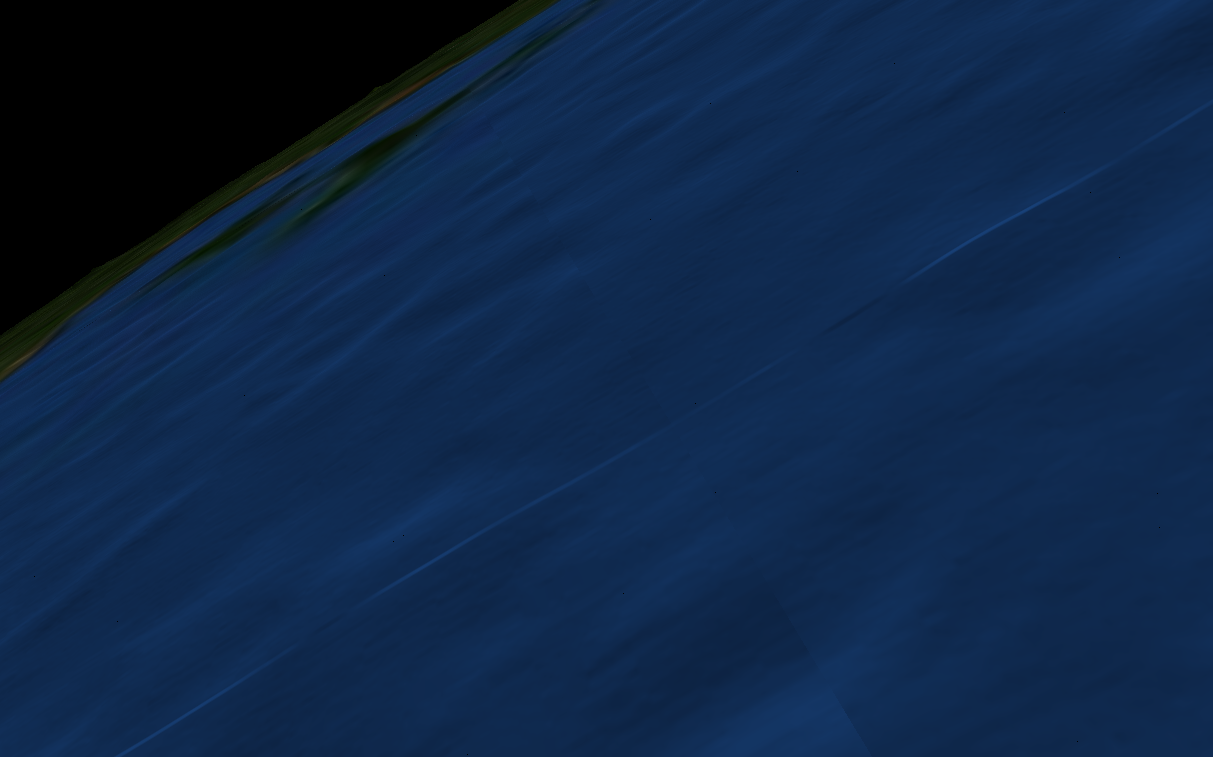
\includegraphics[width=12cm]{img/earth.png}
        \caption{Affichage de la terre}
        \label{fig:earth}
    \end{figure}
    
    
    La figure \ref{fig:earth} présente les deux problèmes majeur, on peut voir dans l'océan les cratères induit par la texture de la lune. On peut aussi remarquer au centre de l'image une discontinuité.\\
    
    \paragraph{Critique} On peut aussi critiquer l'utilisation de textures chargées depuis le disque car ces dernières, à l'instar d'une génération procédurale passe par des pré-traitements et des formats de fichiers avec compression.
    \textbf{TODO : Peut être éclaicir l'image pour mieux distinger les artéfacts}
    
    \begin{figure}
        \centering
        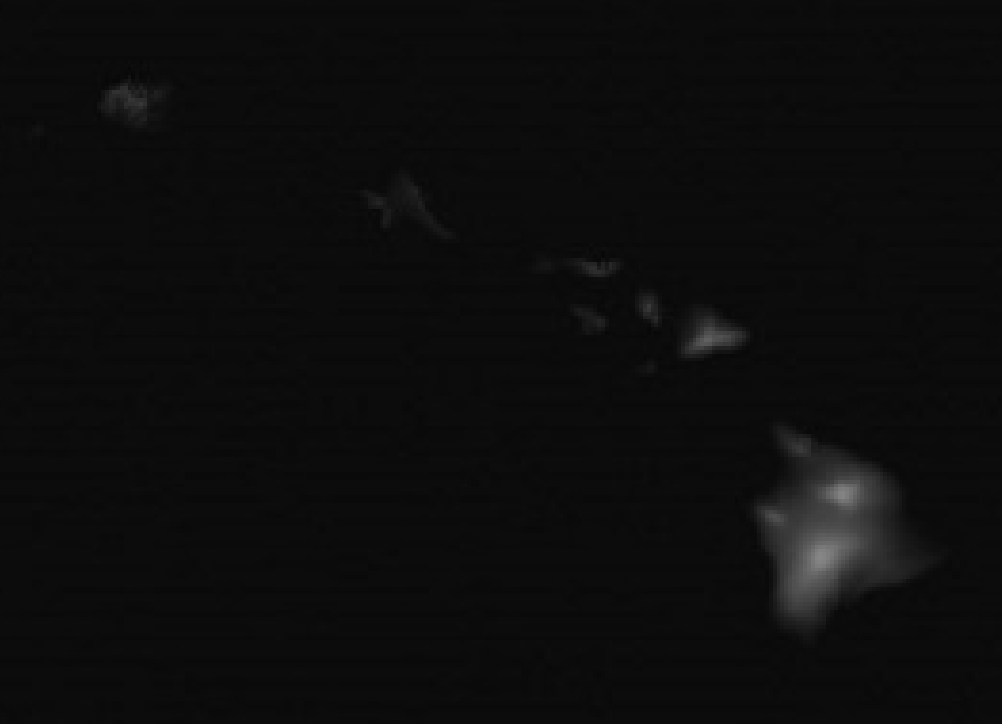
\includegraphics[width=12cm]{img/hawaii.png}
        \caption{Archipel d'Hawaii}
        \label{fig:hawaii}
    \end{figure}
    
    La figure \ref{fig:hawaii} représente l'archipel d'Hawaii extrait de la carte de hauteur de la terre
    (\textit{EarthHeight16k.jpg}). On distingue très clairement des artéfacts dans la partie océan.
    
    \subsection{Travail effectué}
    Une classe Procedural à été écrite, elle permet de créer une planète en utilisant un algorithme de bruit
    sur la texture de la carte de hauteur.
    Des modifications importantes ont été faites dans le code de Texture et dans le shader patch.
    Un nouveau constructeur à été écrit pour prendre en charge ce nouveau type de texture. En effet de 
    base le constructeur reçoit une chaîne de caractère représentant un chemin d'accès sur le disque.
    Ce nouveau constructeur prend quand à lui un tableau à deux dimensions de floattants et sa taille en paramètre.\\
    La méthode $Texture::load$ à aussi été modifié pour permettre l'envoie de ce tableau directement à la carte graphique.\\
    
    \subsection{Correction des problèmes}
    Le problème subsiste lorsque qu'on charge une image depuis le disque mais lorsque l'on génère procéduralement une image,
    il n'y a pas de conversion vers flottant donc pas de problème. Les données sont directement des flottants dispersés sur toute la gamme [-1;1].\\
    De même, comme des données suffisamment précises sont créées, il n'est plus nécessaire de charger des images supplémentaires. Ce qui corrige aussi les problèmes de discontinuités.\\
    L'image doit cependant être générée avec un algorithme de bruit 3d.\\
    
    
    Actuellement encore un bug subsiste, un dépassement de tampon au sein des pilotes graphiques. 
    Les données étant tous le temps dans
    la même page mémoire, le programme ne plante pas. Cependant, les données pointées lors de ce dépassement étant indéfinies, certains sommets pouvaient avoir une hauteur bien supérieur à la normal. Une solution provisoire était de seuiller le sommets dans le shader.\\
    \textbf{TODO Problème corrigé ?}
    
   \section{Génération du maillage}	% Explication de triangulator.
  % icosaèdre ?
  % triangulator ?
  % structure de données
	\subsection{Icosaèdre}
	\label{subsec:icosahedre}
	
	Il existe plusieurs manières de générer un maillage de planète, la méthode utilisé ici
	se base sur un icosaèdre, une forme géométrique composée de douze sommets de base et 
	de vingt faces triangulaire. Chaque face étant un triangle équilatéral de taille identique.
	
	Pour se faire il est nécessaire d'utiliser le nombre d'or $\Phi = \frac{(1+\sqrt(5)}{2}$ , qui est le seul rapport permettant de construire le plus petit deltaèdre ( polyèdre dont les faces sont toutes des triangles équilatéraux).
	
	La méthode utilisé pour former les triangles équilatéraux (et donc l'isosaèdre) et de se servir de 3 plans respectant les proportions du nombres d'or, qui se coupe en leur centre. En reliant les 12 sommets possibles, on va ainsi former les 20 faces de notre icosaèdre, comme on peut l'observer sur la figure \ref{fig:plans-icosaèdre}.
	
	\begin{figure}[H]
        \centerline{
            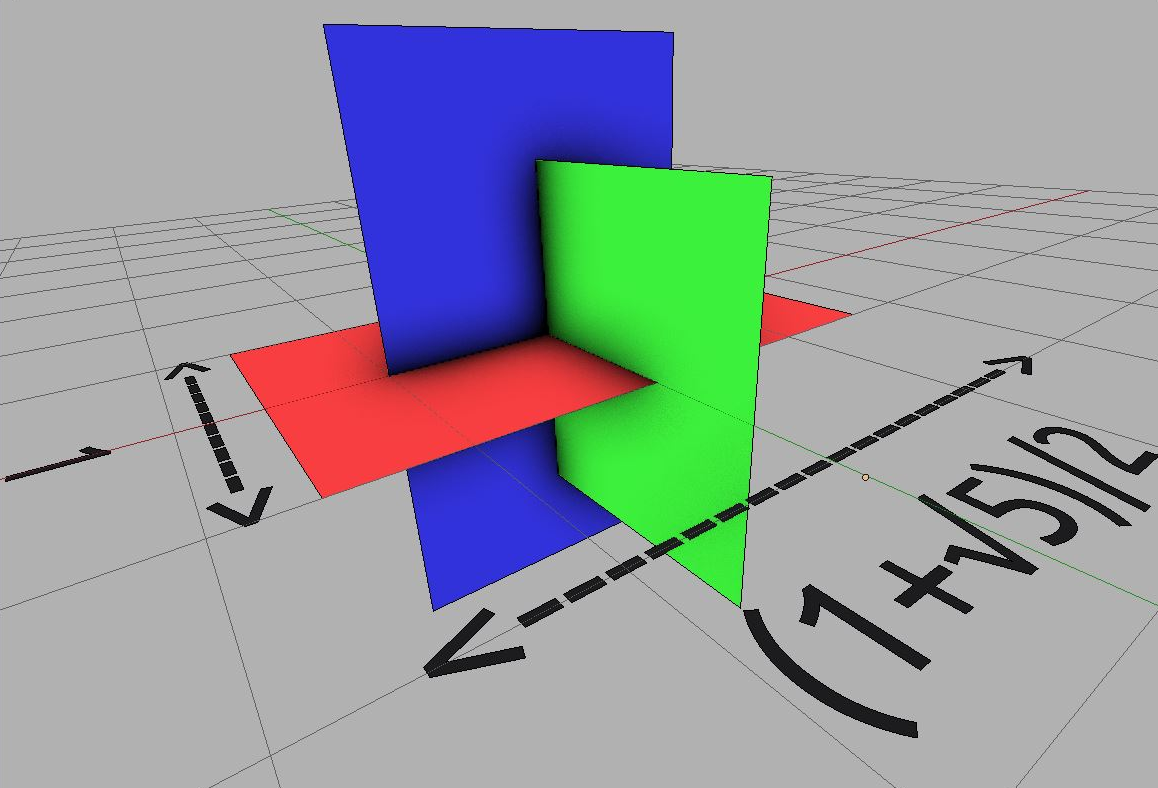
\includegraphics[height=4cm,width=4.5cm]{img/3plans.png}
            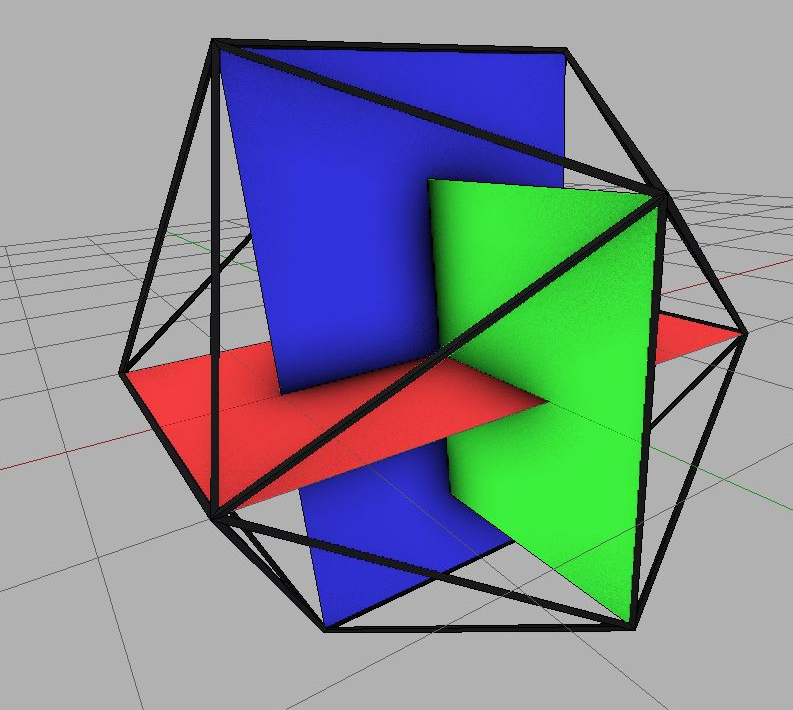
\includegraphics[height=4cm,width=4cm]{img/3plans2.png}}
        \caption{Formation de l'icosaèdre \protect\footnotemark}
        \label{fig:plans-icosaèdre}
	\end{figure}
	\footnotetext{Extrait de \url{http://robert-lindner.com/img/blog/planet_renderer/week5-6/researchPaper.pdf}, dernier accès Mars 2018}
	
	
	% Parler de la generation avec le nombre d'or
	
	La génération du maillage et l'entièreté de la partie LOD de l'algorithme se fait dans la classe Triangulator. L'arbre de données est implémenté avec la méthode des flux du CDLOD (StreamingCDLOD), dont les avantages ont été expliqué précédemment.
	
	L'implémentation ici ne suis pas entièrement le standard du \textit{StreamingLOD}, il a été expliqué que l'algorithme peux conserver les parties qui reste dans le champs de vision. Ici l'intégralité de l'arbre est regénéré à chaque tours de boucle. Cependant dans un contexte de visualisation simple les gains de performances engendrés par de tel optimisations sont négligeables.
	
	Pour accélérer les temps d'accès mémoire, les distances avec les différents triangles sont conservées
	dans un tableau. \\

	Dans l'arbre, chaque noeud possède trois positions correspondant aux trois points du triangle,
	ainsi que quatre pointeurs vers les niveaux suivants.
	D'autre informations sont stockées comme un pointeur vers son parent, le niveau actuelle du
	noeud dans l'arbre ou encore un drapeau correspondant au type du noeud.
	Le drapeau sous forme d'un enum permet de distinguer le noeud qui sont a l'intérieur de l'arbre de ceux
	qui ne le sont pas. Il permet aussi de renseigner si le noeud est une feuille.
		
	Pour chaque triangle, on commence par tester si le triangle est visible, c'est à dire si il est
	présent à l'intérieur du cône de vision de la caméra. Si c'est la cas, on prend le centre de chaque
	arrête du triangle l'on recommence de manière récursive tans que une subdivision est nécessaire.
	C'est à dire tans que le noeud contenant le triangle n'est pas une feuille. Dans le cas contraire,
	
	
    \begin{figure}[!ht]
        \centerline{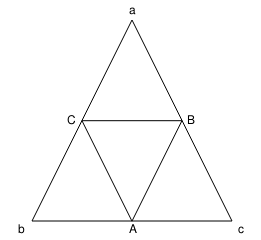
\includegraphics[width=5cm]{img/TriangleSplit.png}}
        \caption{Division}
        \label{fig:TriangleSplit}
    \end{figure}
	
	On peut se rendre compte de la découpe du triangle en quatre plus petit dans la figure 
	\ref{fig:TriangleSplit}.
	Les appels récursifs se font dans l'ordre aBC, AbC, ABc et enfin le triangle du milieux ABC.\\
	
	La méthode SplitHeuristic permet en fonction de trois coordonnées représentant un triangle 
	et du niveau d'établir si ce triangle est dans le cône de vision ou non et de retourner le bon drapeau.
	Les méthodes permettant de déterminer si le cône de vision contient un triangle sont définies dans
	la classe Frustum.
	
  \section{Application du morphing}
  L'algorithme de génération du maillage utilisant le morphing est développé dans la classe \textit{Patch}.\\ 
  
  Le mécanisme du \textit{Patch} est décomposés en deux structures différentes,
  \textit{PatchVertex} et \textit{PatchInstance} et une classe \textit{Patch}.\\
 
  La structure \textit{PatchVertex} permet de stocker les informations relative à un sommet tel que ça position, codé dans un vecteur de taille 3 et le \textit{morphing}, codé dans un vecteur de taille 2. Ces informations sont ensuite envoyé à la carte graphique.
  
  \textbf{TODO PatchInstance}\\
  
  Il ce base sur deux listes appelées m\_Vertices et m\_Indices qui permettent respectivement de stocker des structures \textit{PatchVertex} et des entiers signées.\\
  
  Les informations de positions stockées dans la liste sont envoyées à la carte graphique et permettent de positionner le sommet dans les trois dimensions.\\
  
  La figure \ref{fig:morphTri} représente les transitions du \textit{morphing} lors de l'augmentation du niveaux de détails de la zone.
  	
\begin{figure}[H]
    \centering
    \begin{subfigure}[b]{0.17\textwidth}
       \centering 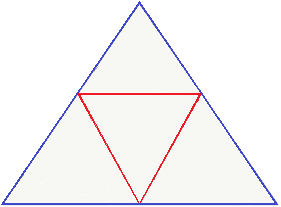
\includegraphics[width=\textwidth,height=2.25cm]{img/morph5.png}
       \caption{}\label{subfig:morph5}
    \end{subfigure}
    ~ 
    \begin{subfigure}[b]{0.17\textwidth}
       \centering 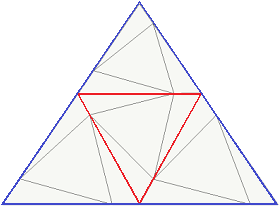
\includegraphics[width=\textwidth,height=2.3cm]{img/morph4.png}
       \caption{}\label{subfig:morph4}
    \end{subfigure}
    ~
    \begin{subfigure}[b]{0.17\textwidth}
       \centering 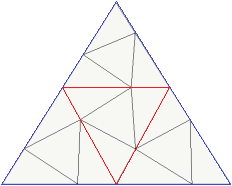
\includegraphics[width=\textwidth,height=2.3cm]{img/morph3.png}
       \caption{}\label{subfig:morph3}
    \end{subfigure}
    ~
    \begin{subfigure}[b]{0.16\textwidth}
       \centering 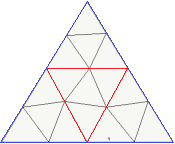
\includegraphics[width=\textwidth,height=2.3cm]{img/morph2.png}
       \caption{}\label{subfig:morph2}
    \end{subfigure}
     ~
    \begin{subfigure}[b]{0.16\textwidth}
       \centering 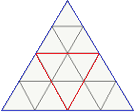
\includegraphics[width=\textwidth,height=2.3cm]{img/morph1.png}
       \caption{}\label{subfig:morph1}
    \end{subfigure}
    \caption{Morph sur des triangles}\label{fig:morphTri}
\end{figure}

    Dans la figure \ref{subfig:morph5}, le triangle Bleu est déjà subdiviser en quatre triangles, et a donc déjà été augmenté en niveau de détails.
    Lorsque l'on change de niveau de détails, chaque triangle concerné est divisé en quatre nouveaux triangles ce qui correspondent à l'ajout de trois nouveaux sommets. Ces nouveaux sommets ont tous d'abord la même position que les trois ancien, il reste à la même hauteur que la face, c'est à dire qu'ils se déplacent en suivant les arêtes du triangle parent jusqu'au milieu de ce dernier.
    Les figures \ref{subfig:morph4}, \ref{subfig:morph3}et \ref{subfig:morph2} représentent le déplacement des sommets, permettant ainsi d'obtenir le triangle Bleu final, à un troisième niveaux de détails visible dans la figure \ref{subfig:morph1}.\\
    
    Les sommets crées sont ainsi relatif au triangle et leur position est représenté en deux dimensions sur le même plan.
  
  Ces informations sont stocker dans le vecteur de taille deux dans la structure \textit{PatchVertex}.\\
  
  
  
  
  \section{Frustum}
  
  Comme dit dans la partie architecture, le frustum a pour but d'éliminer les triangles qui ne sont pas présent dans le cône de vision de la caméra.\\
  La figure \ref{fig:culling} représente ce que voit la caméra (matérialisée par la pointe du cône).
  
  \begin{figure}
  \centering
  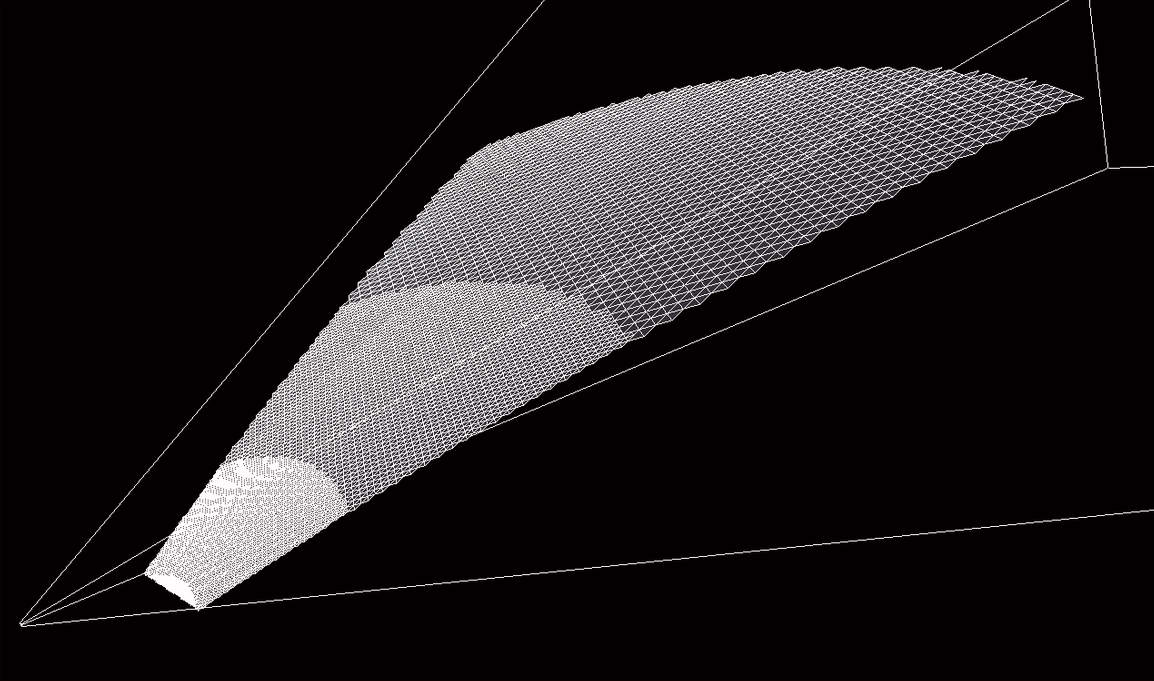
\includegraphics[width=10cm]{img/culling.png}
  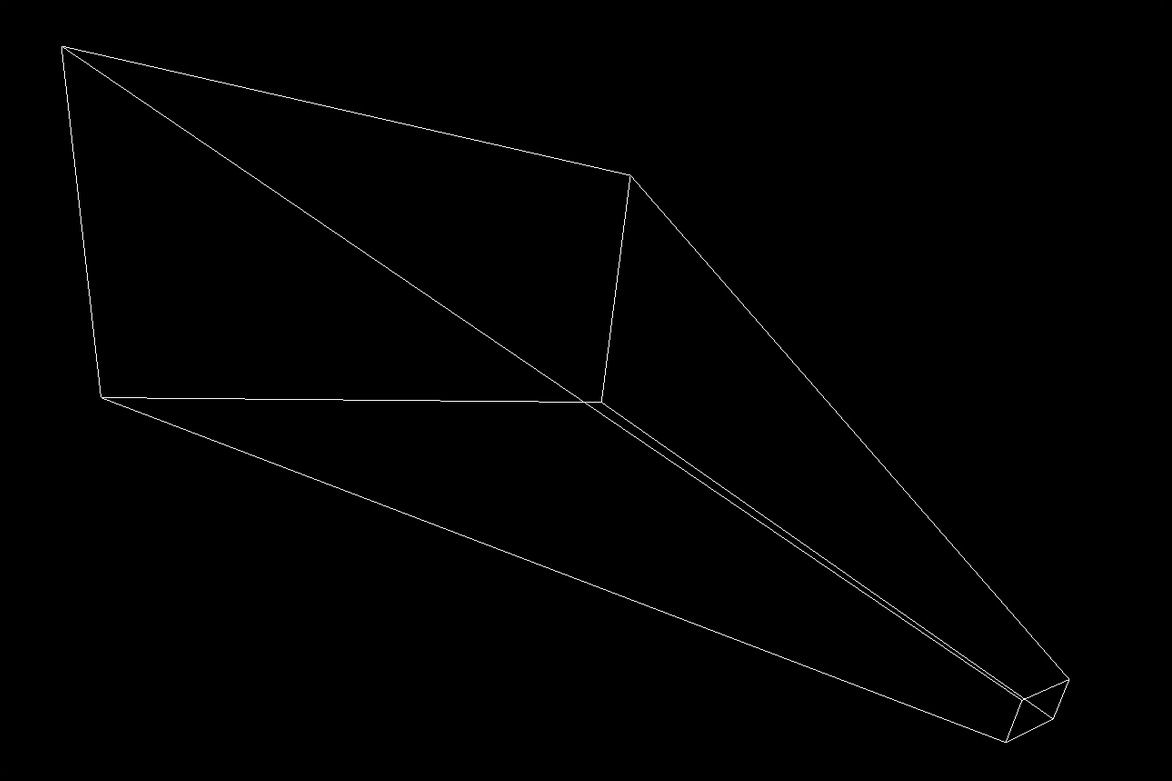
\includegraphics[width=10cm]{img/frustumbox.png}
  \caption{Cône de vision de la caméra \protect\footnotemark}
  \label{fig:culling}
  \end{figure}

  \footnotetext{Extrait de \url{http://robert-lindner.com/img/blog/planet_renderer/week5-6/researchPaper.pdf}, dernier accès Mars 2018}
 
  Le \textit{frustum} est construit autour de six plans différents, quatre représentant les quatre côtés du cône et deux représentant le plan le plus proche et le plan le plus loin.
  On peut voir la structure géométrique du cône de vision dans la figure \ref{fig:culling}
  
  Ces plans sont calculés en fonction de l'angle de vue, de la taille de la fenêtre et des plans \textit{near} et \textit{far}.
  
  \section{Génération de la carte de hauteur}
  
  Dans le code d'origine, les cartes de hauteur était chargée depuis le disque. Nous avons développés un nouveaux type de planète hérité de \textit{Planet} qui permet de générer une planète avec plusieurs types de bruits différents.
  
  Le processus de création de la texture de bruit se base sur un structure contenant les différents paramètre du bruit.
  Chaque bruit étant spécifique, certain nécessite plus de paramètre que d'autre, par exemple un bruit de \textit{simplex} classique à besoin uniquement d'une taille alors qu'un bruit
  de simplex de type \textit{flow noise} utilise d'autres paramètres comme par exemple un octave. 